
This chapter describes algorithms which for a given point set compute
the ``best'' inscribed object from a specific
class. We provide algorithms for
computing maximal inscribed $k$-gons (triangles, quadrilaterals,
\dots) of a planar point set $P$. Maximal $k$-gons are convex, and it
is known that their vertices can be chosen to be vertices of the
convex hull of $P$. Hence, the functions
\ccc{CGAL::maximum_area_inscribed_k_gon_2} and
\ccc{CGAL::maximum_perimeter_inscribed_k_gon_2} operate on convex polygons
only. The example below shows that the largest area triangle (green)
and the largest perimeter triangle (orange, containing the top point)
of a point set are different in general.

\begin{ccHtmlOnly}
<center>
<img border="0" src="max_triangle.gif" align="center">
</center>
\end{ccHtmlOnly} 

\begin{ccTexOnly}
\begin{center}
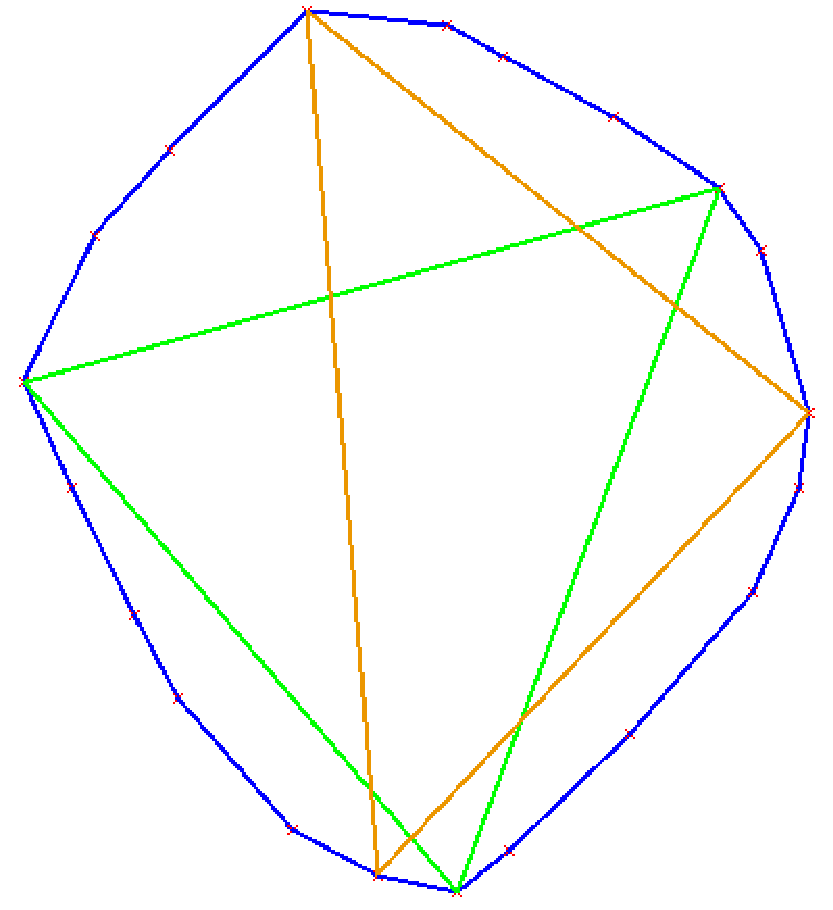
\includegraphics[width=5cm]{Inscribed_areas/max_triangle}
\end{center}
\end{ccTexOnly}


We further provide an algorithm for computing the maximal area
inscribed axis parallel rectangle 

Given a set of points in the plane, the class \ccc{CGAL::Largest_empty_iso_rectangle_2<T>}
is a data structure that maintains an iso-rectangle with the largest area among
all iso-rectangles that are inside a given iso-rectangles, and
that do not contain any point of the point set.

\begin{ccHtmlOnly}
<center>
<img border="0" src="largestEmptyRect.gif" align="center">
</center>
\end{ccHtmlOnly} 

\begin{ccTexOnly}
\begin{center}
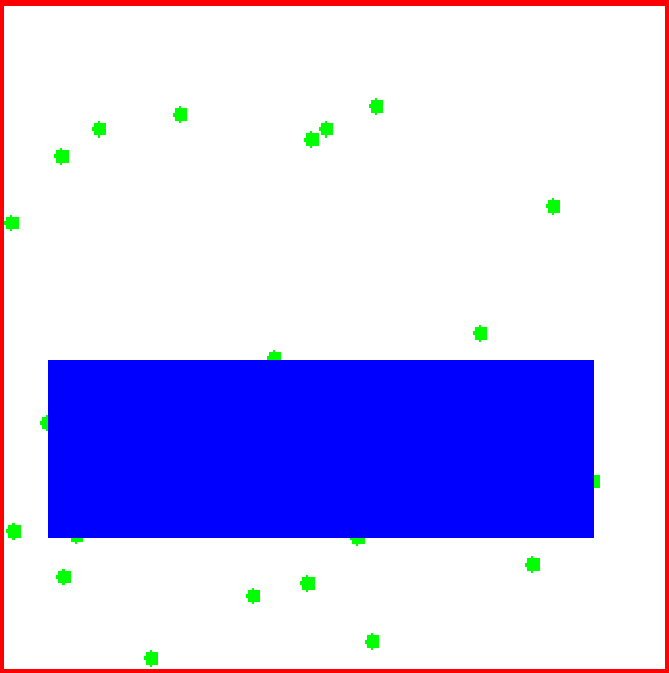
\includegraphics[width=5cm]{Inscribed_areas/largestEmptyRect}
\end{center}
\end{ccTexOnly}

Inscribed volumes are also frequently applied to extract
geometric properties of objects. The largest area triangle is for example used in
heuristics for matching archaeological aerial photographs. Largest
perimeter triangles are used in scoring cross country soaring flights,
where the goal is basically to fly as far as possible, but still
return to the departure airfield. To score simply based on the total
distance flown is not a good measure, since circling in thermals
allows to increase it easily.



